\documentclass{article}

\newcommand{\dir}{~/projects/latex}
\input{\dir/include.tex}
\load{recommended}

\usepackage{tikz}
\usepackage[T1]{fontenc}
\usepackage{imakeidx}
\makeindex

\setup{Linear Algebra}

\begin{document}
\startDocument
\usetcolorboxes
\setcounter{section}{-1}
\setcounter{numberingConfig}{3}

\vspace{3cm}
\begin{Huge}
    \[
        \begin{pmatrix}
            1 & 2 & 3\\
            4 & 5 & 6\\
            7 & 8 & 9
        \end{pmatrix} + 
        \begin{pmatrix}
            9 & 8 & 7\\
            6 & 5 & 4\\
            3 & 2 & 1
        \end{pmatrix} =
        \begin{pmatrix}
            10 & 10 & 10\\
            10 & 10 & 10\\
            10 & 10 & 10
        \end{pmatrix}
    \]
\end{Huge}

\vspace{3cm}
\begin{center}
    \begin{Large}
        ``\textit{Lineare Algebra ist Kulturgut}''
    \end{Large}

    \hspace{3cm} - Robert Weissmantel, 2024
\end{center}

\vspace{3cm}
\begin{center}
    HS2024, ETHZ\\[0.2cm]
    \begin{Large}
        Exam-Summary of the lecture notes
    \end{Large}\\[0.2cm]
    \url{https://ti.inf.ethz.ch/ew/courses/LA24/notes_part_I.pdf} 
    
    and 

    \url{https://ti.inf.ethz.ch/ew/courses/LA24/notes_part_II.pdf}
\end{center}
\newpage

\printtoc{Aquamarine}
\newpage
\newsection
\section{Introduction}
This summary is designed to provide the optimal balance between depth and broadness for the exam. To print this summary, print two pages per A4 paper (so A5 size), leaving out the first three pages (Title page, Table of Contents, Introduction)

The introductory sections were kept as short as possible to allow for more space for the more difficult parts

\newpage
\newsectionNoPB
\section{Vectors}
\label{sec:vectors}
\fhlc{Orange}{\textit{SIMPLIFY RESULTS AS MUCH AS POSSIBLE}} ($21 \div 12 = 7 \div 4$)

\setcounter{all}{4}
\shortdef \textbf{Linear Combination}: $\sum_{i=1}^{n} \lambda_i v_i$, scaled combination of $n$ vectors $v_i$. 

\setcounter{all}{7}
\shortdef It is called an \textbf{Affine Combination} if $\sum_{i=1}^{n} \lambda_i = 1$, a \textbf{Conic Combination} if $\lambda_i \geq 0$ for $i = 1, 2, \ldots, n$ and a \textbf{Convex Combination} if it is affine and conic. Linear combination as a matrix: $Ax = b$, where the matrix's columns are the vectors $v_i$ and $x$'s components are $\lambda_i$
%
\setcounter{all}{9}
\shortdef \textbf{Scalar-Product}: Multiply component wise, add all components together. Results in number, alternatively $v^{\top}w$ (S2.2.3), or $\sum_{i = 1}^{n} v_i w_i$;

\begin{wrapfigure}[10]{l}{0.5\textwidth}
    \includegraphics[width=0.5\textwidth]{/home/janis/NextCloud/Documents/ETH/Semester1/Subjects/LinAlg/Summary/combinations.png}
    \caption{Different kinds of combinations of two vectors}\label{fig:combinations}
\end{wrapfigure}

\textbf{Dot-Free Notation}: Similar to summation notation, we can use it to define e.g. vector addition: $[v_i]_{i=1}^{m} + [w_i]_{i=1}^{m} := [v_i + w_i]_{i=1}^{m}$;
\setcounter{all}{11}\shortdef \textbf{Euclidean Norm}: $||v|| = \sqrt{v \cdot v} = \sqrt{v^{\top}v}$;
\textbf{Squared norm}: $v^{\top}v = ||v||^2$
\textbf{Unit-Vector}: $||v|| = 1$, obtaining: $\frac{v}{||v||} = \frac{1}{||v||} \cdot v$;
\shortlemma \textbf{Cauchy-Schwarz inequality}: $|v \cdot w| \leq ||v|| \cdot ||w||$ for any vectors $v, w \in \R^m$. Equality if $v\lambda = w$ or $w\lambda = v$;
\setcounter{all}{14}\shortdef \textbf{Angles}: $\cos(\alpha) = \frac{v \cdot w}{||v|| \cdot ||w||}$. If $v \perp w \in \R^m$, then $v \cdot w = 0$;
\setcounter{all}{16}\shortlemma \textbf{Triangle inequality}: $||v + w|| \leq ||v|| + ||w||$;
\textbf{Hyperplane}: $\{v \in \R^n : v \cdot d = 0\}$, $d \in \R^n$, $d \neq 0$;
\setcounter{all}{19}\shortlemma \textbf{Linear independence}: Vectors are linearly independent if (a) no vector is a linear combination of the others or (b) there are no $\lambda_i$, such that $\sum_{i = 1}^{n} \lambda_i v_i = 0$. For matrices: $\neg \exists x \neq 0 : Ax = 0$ (no column vector is a linear combination of another).
\setcounter{all}{22}\shortdef \textbf{Span of vectors}: Set of all linear combinations of a vector;
\textbf{Standard Basis vector}: Vector with just one component being $1$, all others $0$;



\newsectionNoPB
\section{Matrices}
\label{sec:matrices}


\textbf{Size}: $m \times n$: $m$ rows, $n$ cols (\textit{\textbf{Z}eilen \textbf{z}uerst, \textbf{S}palten \textbf{s}päter});
\setcounter{all}{2}\shortdef \textbf{Addition}: $A + B := [a_{ij} + b_{ij}]_{i = 1, j = 1}^{m \hspace{3mm} n}$;
\textbf{Scalar-multiple}: $\lambda A := [\lambda a_{ij}]_{i = 1, j = 1}^{m \hspace{3mm} n}$;
\shortdef \textbf{Square matrices}: \textbf{Identity matrix}: quadratic matrix, diagonals $1$, $A = AI = IA$;
\textbf{Diagonal matrix}: $a_{ij} = 0$ if $i \neq j$;
\textbf{Triangle matrix}: \textit{lower} if $a_{ij} = 0$ for $i < j$, \textit{upper} else;
\textbf{Symmetric matrix}: $a_{ij} = a_{ji} \forall i, j$,  $A^{\top} = A$;

\shortdef \textbf{Matrix-Vector-Product}: Rows of matrix ($m \times n$) with vector ($n$ elements), i.e. $u_1 = \sum_{i = 1}^{m} a_{1, i} \cdot v_i$, $Ix = x$;
\textbf{Trace}: Sum of the diagonal entries;

\setcounter{all}{8}\shortdef \textbf{Column Space}: $\{Ax : x \in \R^n\}$, i.e. the span of the column vectors;
\shortdef \textbf{Rank}: $\text{rank}(A) :=$ the number of linearly independent column vectors;
\setcounter{all}{11}\shortdef \textbf{Transpose}: Mirror the matrix along its diagonal. \setcounter{all}{19}\shortlemma $(AB)^{\top} = B^{\top} A^{\top}$, $(A^{\top})^{\top} = A$ (O2.12);
\setcounter{all}{13}\shortdef \textbf{Row Space}: $R(A) = C(A^{\top})$;

\setcounter{all}{16}\shortdef \textbf{Matrix Multiplication}: $A \times B = C$, $c_{ij} = \sum_{k = 1}^{n} a_{i, k} b_{k, j}$. 
Dimension restrictions: $A$ is $m \times n$, $B$ is $n \times p$, result is $m \times p$.
\textit{For each entry, multiply the $i$-th row of $A$ with the $j$-th column of $B$}. \textbf{Not} commutative, but associative \& distributive;
\setcounter{all}{21}\shortlemma \textbf{Outer product}: $\text{rank}(A) = 1 \Leftrightarrow \exists$ non-zero vectors $v \in \R^m$, $w \in \R^n$,
s.t. $A$ is outer product, i.e. $A = vw^{\top}$, thus $\text{rank}(vw^{\top}) = 1$

\textbf{Rotation matrix}: $R(\xi) = \begin{bmatrix}\cos(\xi) & -\sin(\xi)\\ \sin(\xi) & \cos(\xi)\end{bmatrix}$;

\setcounter{all}{23}\shorttheorem \textbf{CR-Decomposition}: $A = CR$. Get $R$ from (reduced) row echelon form, $C$ is the columns from $A$ where there is a pivot in $R$. $C \in \R^{m \times r}, R \in \R^{r \times n}$ (in RREF), $r = \text{rank}(A)$;
\addIndex{Row Echelon Form}: To find REF, try to create pivots: $R_0 = \begin{bmatrix}
    \textcolor{Red}{1} & 0 & 2 & 3\\
    0 & \textcolor{Red}{1} & 2 & 1\\
    0 & 0 & 0 & 0
\end{bmatrix}$, use Gauss-Jordan-Elimination to find it (row-transformations);
\addIndex{Reduced REF}: RREF is simply REF without any zero rows (i.e. in $R_0$, $R$ (in RREF) would be $R_0$ without the last row).

\setcounter{all}{25}\shortdef \textbf{Transformations}: A matrix can be understood as a re-mapping of the unit vectors, scaling and re-orienting them. Each column vector can then be understood as the new unit vector $e_i$, hence essentially adding another coordinate system to the original one, which is moved and rotated a certain way. The rotation matrix under \ref{sec:matrices} is such an example. To prove that $T$ is linear transformation, use: $T(x + y) = T(x) + T(y)$ and $T(\lambda x) = \lambda T(x)$. Then insert the linear transformation given by the task and replace $x$ (or whatever variable there is) with $x + y$ or $\lambda x$. $Ax = \sum_{i=1}^{n}(x_i v_i)$, where $v_i$ is the $i$-th column of $A$;
\setcounter{all}{25}\shortdef \textbf{Kernel}: $\text{Ker}(T) := \{x \in \R^n : T(x) = 0\} \subseteq \R^n$;
\textbf{Image}: $\text{Im}(t) := \{T(x) : x\in \R^n\} \subseteq \R^m$;

\newsectionNoPB
\vspace{-0.5pc}
\section{Solving Linear Equations}
\label{sec:sle}
Put the system of linear equation's factors (i.e. for a linear equation $ax + by + cz = u$, we would put $a, b, c$ into the matrix and $u$ into the vector) into a matrix, where each row is an equation and the result into a vector $b$. Then, we solve $Ax = b$ by Gauss elimination.

\textbf{Gauss elimination}: Transform matrix $A$ into upper triangle matrix by performing row transformations (adding, adding scalar multiples, multiplying by scalar) on it. All operations performed on $A$ have to also be performed on $b$. Typically, write down both as a matrix with a dividing line between $A$ and $b$. Then solve by back-substitution. Gauss elimination succeeds iff $A \in \R^{m \times m}$ and $A$'s columns are linearly independent. (Runtime: \tco{m^3})

\vspace{-0.5pc}
\subsection{Inverse}
\label{sec:inverse}
\setcounter{all}{7}\shortdef{Inverse}: Perform Gauss-elimination on a matrix of form $\begin{bmatrix}A \divides I\end{bmatrix}$ until we get $\begin{bmatrix}I \divides A^{-1}\end{bmatrix}$. $A$ is invertible, iff $\det(A) \neq 0$. Alternative: $MM^{-1} = M^{-1}M = I$. $M$ has to be square. $0$ matrix has no inverse

\textbf{Inverse for specific sizes}: $1 \times 1$ $M = \begin{bmatrix}a\end{bmatrix}, M^{-1} = \begin{bmatrix}\frac{1}{a}\end{bmatrix}$ (if $a \neq 0$); $2\times2$ $M = \begin{bmatrix}a & b\\ c & d\end{bmatrix}$ $M^{-1} = \frac{1}{\text{det}(M)}\begin{bmatrix}d & -b\\ -c & a\end{bmatrix}$;
\setcounter{all}{9}\shortlemma \textbf{Inverse product}: $(AB)^{-1} = B^{-1} A^{-1}$;
\shortlemma $(A^{-1})^{\top} = (A^{\top})^{-1}$;
\shorttheorem \textbf{Inverse theorem}: $A$ is invertible $\Leftrightarrow$ $Ax = b$ has a unique solution $\forall b \in \R^n$ $\Leftrightarrow$ the columns of $A$ are independent. \textbf{Diagonal matrix}: each element reciprocal. (Might require proof)

\vspace{-0.5pc}
\subsection{LU-Decomposition}
\label{sec:lu-decomp}
\setcounter{all}{13}\shorttheorem \textbf{LU-Decomposition}: $A = LU$. $U$ upper triangle, result of Gauss elimination, $L$ lower triangle, $(E_1 \times E_2 \times \ldots \times E_n)^{-1}$.
Transformation matrices $E$ ($E \cdot A = A_1$): transformation is a single entry in lower triangle, where the $i$ and $j$ are the two rows involved and the value of $e_{ij}$ is the operation performed on the two. $L^{-1}$ for size $3$: Diagonal, $L^{-1}_{1,2} = -L_{1,2}$, $L^{-1}_{2,3} = -L_{2,3}$, $L^{-1}_{1,3} = -L_{1,3}$.
When multiplying up to three different ones, copies values to multiplied matrix.
If it is impossible to decompose $A$ into $LU$ without row exchanges, we get $PA = LU$, where $P$ is a permutation matrix (indicating which rows have been swapped). Time complexity is improved significantly with this \tco{m^2}.

\shortdef \textbf{Permutations}: bijective function $\pi$ on matrix; Reorders the input structure (i.e. vector or matrix); 
\shortdef \textbf{Permutation matrix}: $p_{ij} = \begin{cases}
    1 & \text{if } j = \pi(i)\\
    0 & \text{else}
\end{cases}$
\shortlemma $P^{-1} = P^{\top}$. 

\setcounter{all}{18}\shorttheorem \textbf{LUP-Decomposition}: $PA = LU$, where $U = P\times L A$. $P_j = I$ if no row swaps are performed at each step and $P = P_m \times P_{m - 1} \times \ldots \times P_1$. Rewriting this as $A = P^{\top}LU$, we can simply solve an SLE using LUP-Decomposition

\vspace{-0.5pc}
\subsection{Gauss-Jordan-Elimination}
\label{sec:gauss-jordan}
\textbf{Gauss-Jordan-Elimination}: Generalization of Gauss elimination to $m \times n$ matrices, still works similarly to Gauss elimination. We aim to find REF or RREF (see \ref{sec:matrices}). To describe, we say REF$(j_1, j_2, \ldots, j_r)$ or equivalently with RREF, where $j_r$ is the $r$-th pivot.

The solution is then in a vector, whose components are either $0$ or the $r$-th component of $b$. Example:
\[
    \begin{bmatrix}
        0 & 1 & 0 & 0 & 2 & 0\\
        0 & 0 & 1 & 0 & 3 & 0\\
        0 & 0 & 0 & 1 & 2 & 0\\
        0 & 0 & 0 & 0 & 0 & 1\\
        0 & 0 & 0 & 0 & 0 & 0
    \end{bmatrix}
    \cdot
    \begin{bmatrix}
        0\\b_1\\b_2\\b_3\\0\\b_4
    \end{bmatrix}
    =
    \begin{bmatrix}
        b_1\\b_2\\b_3\\b_4\\\textcolor{Green}{0}
    \end{bmatrix}
\]
If the green marked entry in $b$ were not to be $0$, then the SLE would not have a solution. 


\textbf{CR-Decomposition}: see \ref{sec:matrices} for exaplanation. \setcounter{all}{24}\shorttheorem is described there


\newsection
\section{The four fundamental subspaces}
\vspace{-0.2pc}
\subsection{Vector space}
\vspace{-0.5pc}
\shortdef \textbf{Vector space}: Abstract mathematical concept, elements are vectors; Two operations ($\oplus / +$ and $\odot / \cdot$ (depending on notation)); Triple $(V, +, \cdot)$, $V$ is a set of vectors, satisfying the vector space axioms \textit{commutativity, associativity, existance of zero and negative vectors and identity element ($1$), compatibility of $\oplus$ with $\cdot$ (in $\R$), distributivity over $\oplus$ ($\lambda(v + w) = \lambda v + \lambda w$)} and distributivity over + (in $\R$) ($(\lambda + \mu)v = \lambda v + \mu v$).

\textbf{Defining a vector space}: We need to define addition and scalar multiplication for the elements in a \textbf{\textit{canonical}} way (= \textit{according to accepted standard})

\setcounter{all}{8}\shortdef \textbf{Subspaces}: Two subset axioms, $v + w \in U$, $\lambda v \in U$, 
$\lambda \in \R$ (closed under addition \& scalar multiplcation), where $U \subseteq V$, \shortlemma at least \textbf{\textit{always}} contains the zero vector ($0 \in U$);
$C(A) = \{Ax : x \in \R^n\}$ is a subspace of $\R^m$, if $A \in \R^{m \times n}$;
\setcounter{all}{12} \shortlemma $U$ is also a vector space with the same $+$ and $\cdot$ as $V$;
$U \cap W$ is subspace, $U \cup W$ not;

\bg{Aquamarine}{Prove of vector space / subspace}: Use the axioms and prove each and every one of them, then, if that is successful, conclude that is subspace / vector space.
\setcounter{all}{15}\shortdef \textbf{$\text{Span}(G)$}: Set of all linear combinations of $G$, $G \subseteq V$. Set is \textbf{linearly independent} if no vector $v \in G$ is a linear combination of $G\backslash \{v\}$. Vectors are not linearly independent if non-trivial linear combination of them is $0$-vector

\shortdef \textbf{Basis}: Set of vectors that are linearly independent and span $B$ (number equals dimension of space), subspace of $V$. For $\R^m$, the set of unit vectors is a basis. For a matrix, all linearly independent columns form a basis of the column space $C(A)$. Every set of $m$ linearly independent vectors is a basis of $\R^m$. \textbf{\textit{Calculating:}} If we have a matrix with full column / row rank, then the basis are all column / row vectors.

\setcounter{all}{19} \shortlemma \textbf{Steiniz exchange lemma}: Let $F \subseteq V$ be a finite set of linearly independent vectors, $G \subseteq V$ a finite set of vectors with $\text{Span}(G) = V$. Then: $|F| \leq |G|$, $\exists$ subset $E\subseteq G$ of size $|G| - |F|$ s.t. $\text{Span}(F\cup E) = V$. \shorttheorem $B, B'\subseteq V$, finite bases of $V$, then $|B| = |B'|$;
\shortdef \textbf{Finitely generated vector space}: $\exists G \subseteq V$ with $\text{Span}(G) = V$. \shorttheorem If $V$ finitely generated, then $V$ has a basis $B \subseteq G$.

\shortdef \textbf{Dimension}: $V$ finitely generated, then $d = \dim(V)$ is the size of any basis $B$ of $V$. \shortlemma Let $F \subseteq V$ be a set of $d$ linearly independent vectors, then $F$ is basis of $V$. Let $G$ be a set of $d$ vectors with $\text{Span}(G) = V$, then $G$ is a basis of $V$


\vspace{-0.5pc}
\subsection{Computing the fundamental subspaces}
Let $M$ be an invertible $m \times m$ matrix.

\textbf{Column Space}: Set of all linearly indep. columns ($C(A) = \{Ax : x \in \R^n\} \subseteq \R^m$. 
\shorttheorem The number of pivots in REF form of matrix $A$ is the $\text{rank}(A) = \dim(C(A))$. 
The column vectors at the pivots form the basis of $A$;

\textbf{Row Space}: $R(A) = C(A^{\top}) \subseteq \R^n$. 
\setcounter{all}{27}\shortlemma $R(A) = R(MA)$. \shorttheorem $\dim(R(A)) = \text{rank}(A)$ 
\shorttheorem $\text{rank}(A) = \text{rank}(A^{\top})$;
The rows in RREF form a basis of $A$;

\setcounter{all}{31}\shortdef \textbf{Null Space}: $N(A) = \text{Ker}(A) = \{x \in \R^n : Ax = 0\}$. \shortlemma $N(A) \subseteq \R^n$. 
\shortlemma $N(A) = N(MA)$.
Can be easily obtained from RREF by setting $b = 0$ in $Rx = b$.
If there are any free variables, choose any real (or complex) number satisfying the condition.
\textbf{To find basis}, we can rewrite and apply below Lemma

$Rx = 0 \Leftrightarrow I \cdot x(I) + Q \cdot x(Q) = 0$, e.g. for $R = \begin{bmatrix}
    1 & 2 & 0 & 3\\
    0 & 0 & 1 & -2\\
\end{bmatrix}$ to $I \begin{bmatrix}
    x_1\\ x_3
\end{bmatrix} + \begin{bmatrix}
    2 & 3\\
    0 & -2
\end{bmatrix}
\begin{bmatrix}
    x_2\\x_4
\end{bmatrix} = 0 \Leftrightarrow x(I) = -Q\cdot x(Q)$
We may then freely choose the \textit{free variables} $x(Q)$, then find \textit{basic variables} $x(I)$ using the above, typically choose $e_1, \ldots, e_k$ for $x(Q)$ to get the $k$-the vec of basis ($k =$ num cols of $Q$). 
Finally combine the vectors into one.

\shortlemma $N(R) = N(A)$. The vectors obtained from the above procedure form a basis of $N(R)$

\vspace{-0.3pc}
\shorttheorem $\dim(N(A)) = n - \text{rank}(A)$;


\shortdef \textbf{Left Nullspace}: $LN(A) := N(A^{\top}).$ \shortlemma $LN(A)\subseteq \R^m$. \shorttheorem $\dim(LN(A)) = m - \text{rank}(A)$

\shortdef \textbf{Solution space}: Set of all solutions of $Ax = b$, thus $\text{Sol}(A, b) := \{x \in \R^n : Ax = b\} \subseteq \R^n$. \shorttheorem Let $s$ be some solution of $Ax = b$, then $\text{Sol}(A, b) = \{s + x : x \in N(A)\}$. This means, we can also compute $\text{Sol}(A, b)$ despite it not being a subspace. To describe all solutions, we simply need \textit{some} solutions.

\shortlemma Let $A \in \R^{m \times n}$. If $\text{rank}(A) = m$, $Ax = b$ has a solution for every $b \in \R^m$


% Part II
\newsection
\setcounter{numberSubsections}{1}
\section{Orthogonality}
\subsection{Definition}
\shortdef \textbf{Orthogonality}: Two vectors are orthogonal, if the their scalar product is $0$, i.e. $v^{\top}w = \sum_{i = 1}^{n} v_i w_i = 0$. 
\shortlemma Two subspaces are orthogonal to each other if for each $v \in V$ and $w \in W$, $v$ and $w$ are orthogonal. 
\shortlemma As a consequence, if that is true, all these vectors are linearly independent. 
\shortcorollary $V \cap W = \{0\}$ and their union is $V \cup W = \{\lambda v + \mu w : \lambda, \mu \in \R, v \in V, w \in W\}$. 
If $\dim(V) = k$ and $\dim(W) = l$, then $\dim(V\cup W) = k + l \leq n$, for $V, W \subseteq \R^n$;

\shortdef \textbf{Orthogonal complement}: $V^{\bot} := \{w \in \R^n : w^{\top}v = 0, \forall v \in V\}$. 
\shorttheorem $N(A) = C(A^{\top})^{\bot} = R(A)^{\bot}$ and $C(A^{\top}) = N(A)^{\bot}$.
\shorttheorem The following is equivalent for orthogonal subspaces of $\R^n$: $W = V^{\bot} \Leftrightarrow \dim(V) + \dim(W) = n \Leftrightarrow u = v + w \forall u \in \R^n$ with unique vectors $v \in V, w \in W$. \shortlemma $V = (V^{\bot})^{\bot}$.
\shortcorollary $N(A) = C(A^{\top})^{\bot}$ and $C(A^{\top}) = N(A)^{\bot}$
\shorttheorem $\{x \in \R^n : Ax = b\} = x_1 + N(A)$, where $x_1 \in \R(A)$ such that $Ax_1 = b$
\shortcorollary $N(A) = N(A^{\top}A)$ and $C(A^{\top}) = C(A^{\top}A)$

\newsectionNoPB
\subsection{Projections}
\shortdef \textbf{Projection}:
Projecting a vector onto a subspace is done with $\displaystyle \text{proj}_S(b) = \text{argmin}_{p\in S} ||b - p||$ and yields the closest point (or vector) in the new subspace $S$
\shortlemma \textbf{1-Dimensional}: $\displaystyle \text{proj}_S(b) = \frac{aa^{\top}}{a^{\top}a}b$, where we project $b \in \R^m$ on $S = \{\lambda a : \lambda \in \R\} = C(a)$ where $a \in \R^m\backslash\{0\}$.
We note that $(b - \text{proj}_S(b)) \perp \text{proj}_S(b)$, i.e. the ``error-vector'' is perpendicular to $a$.

\shortlemma \textbf{General case}: PREFER 5.2.6! $S$ is a subspace in $\R^m$ with $\dim(S) = n$.
Let $a_1, a_2, \ldots, a_n$ be a basis of $S$, i.e. $S = \text{Span}(a_1, \ldots, a_n) = C(A) = \{A\lambda : \lambda \in \R^n\}$ where $A$ is a matrix with column vectors $a_1, \ldots, a_n$.
We project $b \in \R^m$ onto the subspace $S$, then $\text{proj}_S(b) = A\hat{x}$, where $\hat{x}$ satisfies $A^{\top}A\hat{x} = A^{\top}b$.
\shortlemma $A^{\top}A$ is invertible $\Leftrightarrow A$ has linearly independent columns $\Rightarrow$ \shortcorollary $A^{\top}A$ is square, invertible and symmetric.

\shorttheorem Projection in terms of projection matrix $P = A(A^{\top}A)^{-1}A^{\top}$: $\text{proj}_S(b) = Pb$, $A$ is the matrix of task

% Page 13 now
\newsectionNoPB
\subsection{Least squares, Linear regression}
\textbf{Least squares}: Approximate a solution to System of equations.
Concept $\displaystyle \min_{\hat{x} \in \R^n} ||A\hat{x} - b||^2$.
Using the normal equations, we get $A^{\top}A\hat{x} = A^{\top}b$.
Using the definition of $\hat{x} = (A^{\top}A)^{-1}A^{\top}b$ to solve the least squares problem borders insanity, so use $A^{\top}A\hat{x} = A^{\top}b$ to solve.
\begin{usage}[]{Least squares}
    \begin{enumerate}[label=(\roman*)]
        \item Calculate $M = A^{\top}A$ (matrix)
        \item Calculate $b' = A^{\top}b$ (vector)
        \item Solve resulting System of Equations $M\hat{x} = b'$ normally
    \end{enumerate}
\end{usage}

\textbf{Linear regression}: Application of least squares problem, problem is to find $A$ and $b$ such that we can solve the system.
We define a matrix
$A = \begin{bmatrix}
        1      & t_1    \\
        \vdots & \vdots \\
        1      & t_n
    \end{bmatrix}$
and a result vector
$b = \begin{bmatrix}
        b_1 \\\vdots\\b_n
    \end{bmatrix}$
where $n$ is the total number of data points and $t_i$ is the slope of the $i$-th function, where $b_i$ is its output.
The first column is all $1$s because the constant element has no scalar, for obvious reasons.
This comes from the following concept: $f(t) = \alpha_0 + \alpha_1 t$, so if the first data point is $(1, 2)$, we get $\alpha + \alpha_1 \cdot 1 = 2$, which we will then transform into a SLE with other equations.

\setcounter{all}{2}\shortlemma The columns in $A$ are linearly dependent $\Leftrightarrow t_i = t_j \hspace{0.2em} \forall i \neq j$


\newsectionNoPB
\subsection{Gram Schmidt}
\shortdef \textbf{Orthonormal vector}: Orthogonal and norm is $1$.
Alternatively: $q_i^{\top}q_j = \delta_{ij}$, \textbf{\textit{Kronecker delta}} $\delta_{ij} = \begin{cases}
        0 & \text{if } i \neq j \\
        1 & \text{if } i = j
    \end{cases}$;
\setcounter{all}{3}\shortdef \textbf{Orthogonal matrix}:
If $Q^{\top}Q = I$, $QQ^{\top} = I$ (if $Q$ square), so $Q^{-1} = Q^{\top}$, columns of $Q$ form orthonormal basis for $\R^n$. \shortex \hspace{0mm} Rotation \& permutation matrices. \setcounter{all}{6}\shortproposition Orthogonal matrices preserve norm and inner product of vectors.
If $Q\in \R^{n \times n}$, then $\forall x, y \in \R^n$, $||Qx|| = ||x||$ and $(Qx)^{\top}(Qy) = x^{\top}y$;
Product of any two orthogonal matrices is orthogonal; For $Q$ orthogonal, we want $a \cdot b + c \cdot d = 0$

\textbf{Projections with orthonormal bases}: Much simpler, because $A^{\top}A = I$ if $A$ has orthonormal columns.
\shortproposition The least squares solution to $Qx = b$, where $Q$ is the matrix whose columns are the vectors forming the orthonormal base of $S \subseteq \R^m$, is given by $\hat{x} = Q^{\top}b$ and the projection matrix is given by $QQ^{\top}$;

\setcounter{all}{9}\shortdef \textbf{Gram-Schmidt}: Used to construct orthonormal bases. We have linearly independent vectors $a_1, \ldots, a_n$ that span a subspace $S$, then Gram-Schmidt constructs $q_1, \ldots, q_n$ by setting $q_1 = \frac{a_1}{||a_1||}$ and for $k = 2, \ldots, n$, $q'_k = a_k - \sum_{i = 1}^{k - 1} (a_k^{\top}q_i) q_i$ then setting $q_k = \frac{q'_k}{||q'_k||}$;

\setcounter{all}{11}\shortdef \textbf{QR-Decomposition}: $A = QR$, where $R = Q^{\top}A$ and $Q$ is obtained from the Gram-Schmidt process, it is made up of the vectors $q_i$ as columns. \shortlemma $R$ is upper triangle and invertible. $QQ^{\top}A = A$, meaning $A = QR$ is well-defined. \shortfact This greatly simplifies calculations involving projections and least squares, since $C(A) = C(Q)$, so $\text{proj}_{C(A)}(b) = QQ^{\top}b$ and for least squares, we have $R\hat{x} = Q^{\top}b$. This can efficiently be solved because $R$ is triangular using back-substitution.


\newsectionNoPB
\subsection{Pseudoinverse}
\textbf{Pseudoinverse}: $A^+ = (A^{\top}A)^{-1}A^{\top}$; $\text{rank}(A) = \text{rank}(A^+)$

Let $A \in \R^{m \times n}$;
\shortdef \textbf{Full column rank}: $\text{rank}(A) = n$. $A^+ = (A^{\top}A)^{-1}A^{\top}$.
\shortproposition $A$ full column rank, $A^+A = I_n$ (left inverse);
\shortdef \textbf{Full row rank}: $\text{rank}(A) = m$. $A^+ = AA^{\top}(AA^{\top})^{-1}$.
\shortlemma $A$ full row rank, $AA^+ = I_m$;
\shortlemma For any matrix $A$ and vector $b \in C(A)$, the unique solution for the least squares problem is given by vector $\hat{x} \in C(A^{\top})$ and satisfies $A\hat{x} = b$.
\shortproposition For a full row rank matrix $A$, the solution is given by $\hat{x} = A^+ b$ with $A\hat{x} = b$;
\shortdef \textbf{General case}: $A^+ = R^+ C^+ = R^{\top}(C^{\top}AR^{\top})^{-1}C^{\top}$.
We can use any full-rank factorization, not just $CR$, i.e. \setcounter{all}{9}\shortproposition let $S\in \R^{m \times r}$ and $T \in \R^{r \times n}$ s.t. $A = ST$, then $A^+ = T^+S^+$.

\setcounter{all}{11}\shorttheorem \textbf{Properties of Pseudoinverse}: $AA^+A = A$, $A^+AA^+ = A^+$, $AA^+$ is symmetric, it is the projection matrix for projections on $C(A)$. $A^+A$ is symmetric, and is the projection matrix on $C(A^{\top})$. $(A^{\top})^+ = (A^+)^{\top}$;


\newsectionNoPB
\subsection{Farka's Lemma \& Projections of sets}
\setcounter{all}{7}\shorttheorem \textbf{Farka's Lemma} Let $A \in Q^{m \times m}$, $b \in Q^m$. There either:
\begin{itemize}
    \item exists a vector $x \in \R^n$ such that $Ax \leq b$ or
    \item there exists a vector $y \in \R^m$ such that $y \geq 0, y^{\top}A = 0$ and $y^{\top}b < 0$
\end{itemize}


\newsection
\section{Determinant}
\label{sec:determinants}
\setcounter{numberingConfig}{4}
\begin{definition}[]{Determinant}
    The determinant can be understood as a number that corresponds to how much the associated linear transformation inflates space, it corresponds to the area of the unit cube, which can be scaled by a matrix operation.
\end{definition}
\setcounter{numberingConfig}{3}

\fhlc{Aquamarine}{$2 \times 2$ matrices} Let $A = \begin{bmatrix}a & b\\c & d\end{bmatrix}$, then $\det(A) = \begin{vmatrix}a & b\\c & d\end{vmatrix} = ad - bc$.

\fhlc{Aquamarine}{$n \times n$ matrices} Can be solved using the Triangle rule, Cramer's Rule, Co-Factors or LU-Decomposition ($\det(A) = \det(LU) = \det(L) \cdot \det(U)$, whereas $L$ and $U$ are triangle matrices, so $\det(U)$ is just the product of all entries on the main diagonal, see properties below)

\setcounter{all}{8}
\begin{properties}[]{Determinant}
    \begin{enumerate}[label=(\Roman*)]
        \item \shortproposition Matrix $T \in \R^{n \times n}$ is triangular, $\det(T) = \prod_{k = 1}^{n}T_{kk}$, in particular, $\det(I) = 1$
        \item \shorttheorem Matrix $A \in \R^{n \times n}$ then $\det(A) = \det(A^{\top})$
        \item \shortproposition Matrix $Q \in \R^{n \times n}$ orthogonal $\Leftrightarrow \det(Q) = 1$ or $\det(Q) = -1$
        \item \shortproposition Matrix $A \in \R^{n \times n}$ invertible $\Leftrightarrow \det(A) \neq 0$
        \item \shortproposition Matrices $A, B \in \R^{n \times n}$, then $\det(AB) = \det(A)\cdot \det(B)$, in particular, $\det(A^n) = \det(A)^n$
        \item \shortproposition Matrix $A \in \R^{n \times n}$, then $\det(A^{-1}) = \displaystyle\frac{1}{\det(A)}$
        \item $\det(2A) = 2^n \det(A)$
    \end{enumerate}
\end{properties}

\shortex \hspace{0mm} \textbf{Triangle rule}: Number of permutations: $n!$. Use diagonals to calculate:
\[
    \det(A) = \begin{bmatrix}
        A_{11} &        &        \\
               & A_{22} &        \\
               &        & A_{33}
    \end{bmatrix}+
    \begin{bmatrix}
               &        & A_{13} \\
        A_{21} &        &        \\
               & A_{23} &
    \end{bmatrix}+
    \begin{bmatrix}
               & A_{12} &        \\
               &        & A_{23} \\
        A_{31} &        &
    \end{bmatrix}
    \text{ and } A = \begin{bmatrix}
        A_{11} & A_{12} & A_{13} \\
        A_{21} & A_{22} & A_{23} \\
        A_{31} & A_{32} & A_{33}
    \end{bmatrix}
\]
and the same the oposite direction (instead of top left to bottom right, top right to bottom left) and subtract that.
\textbf{Don't forget brackets}. Written out, we have
\begin{align*}
    \det(A) = A_{11} A_{22} A_{33} + A_{13} A_{21} A_{23} + A_{12} A_{23} A_{31} - (A_{13} A_{22} A_{31} + A_{12} A_{21} A_{33} + A_{11} A_{23} A_{32})
\end{align*}

\shortdef \textbf{Co-Factors}: $C_{ij} = (-1)^{i + j}\det(\mathscr{A}_{ij})$, where $\mathscr{A}$ is the $(n - 1) \times (n - 1)$ matrix that is obtained when removing the $i$-th row and $j$-th column from $A$. Or more simple: In a $3 \times 3$ matrix, the co-factor are the entries on its first row, $A_{ij}$ the matrix obtained from $A$ without the first row and column $j$ (i.e. the one on which the current co-factor is)
\shortproposition Using this, $\det(A) = \displaystyle\sum_{j = 1}^{n} A_{ij} C_{ij}$.

\shortproposition What we had found as the inverse for $A \in \R^{2 \times 2}$ (see \ref{sec:inverse}) has a form in $\R^{n \times n}$, where $A^{-1} = \frac{1}{\det(A)}C^{\top}$, where $C$ is an $n \times n$ matrix containing the co-factors of $A$ as entries. This can be rewritten as $AC^{\top} = \det(A)I$;

\setcounter{all}{19}\shortproposition \textbf{Cramer's Rule}: The idea here is that we solve a linear system of type $Ax = b$, then using that the detminant is multiplicative, we get $\det(A)x_1 = \det(\mathscr{B}_1)$, where $\mathscr{B}$ is the matrix obtained from $A$ by replacing the first column with $b$. So, the solution $x \in \R^n$ for $Ax = b$ is given by $x_j = \displaystyle \frac{\det(\mathscr{B}_j)}{\det(A)}$

\newsection
\section{Eigenvalues and Eigenvectors}
\setcounter{subsection}{-1}
\subsection{Complex numbers}
\textbf{Operations}: $i^2 = -1$ (NOT $i = \sqrt{-1}$ bc. otherwise $1 = -1$). Complex number $z_j = a_j + b_ji$. \textit{Addition, Subtraction} $(a_1 \pm a_2) + (b_1 \pm b_2)i$. \textit{Multiplication} $(a_1 a_2 - b_1 b_2) + (a_1 b_2 + a_2 b_1)i$. \textit{Division} $\displaystyle\frac{a_1 b_1 + a_2 b_2}{b_1^2 + b_2^2} + \frac{a_2 b_1 - a_1 b_2}{b_1^2 b_2^2}i$;

\textbf{Parts}: $\mathfrak{R}(a + bi) := a$ (Real part), $\mathfrak{I}(a + bi) := b$ (imaginary part), $|z| := \sqrt{a^2 + b^2}$ (modulus), $\overline{a + bi} := a-bi$ (complex conjugate);
\setcounter{all}{2}\shortfact\textbf{Polar coordinates}: $a + bi$ (normal form), $r \cdot e^{i \phi}$ (polar form). Transformation polar $\rightarrow$ normal: $r \cdot \cos(\phi) + r \cdot \sin(\phi)i$. Transformation normal $\rightarrow$ polar: $|z| \cdot e^{i \cdot \arcsin(\frac{b}{|z|})}$;
\textbf{Conjugate Transpose}: $A^* = \overline{A}^{\top}$ (also knows as \textit{hermitian transpose});

\shorttheorem \textbf{Fundamental Theorem of Algebra}: Any polynomial of degree $n \geq 1$ has a zero $\lambda \in \C$ s.t. $P(\lambda) = 0$, precisely, $n$ zeros (=roots). The number of times a certain $\lambda$ appears is called the \textit{algebraic multiplicity}.

\textbf{Complex valued matrices and vectors}: Works very similar to with real numbers, but the transpose has to be replaced by the conjugate transpose.


\newsectionNoPB
\subsection{Eigenvalues \& Eigenvectors}
\begin{definition}[]{Eigenvalues \& Eigenvectors}
    We call $\lambda \in \C$ an eigenvalue of $A \in \R^{n\times n}$ and $v \in \C^n\backslash\{0\}$ an eigenvector of $A$ if $Av = \lambda v$. 
    The two are then called an eigenvalue-eigenvector pair and if $\lambda \in \R$, then it is a real eigenvalue and we have a real eigenvalue-eigenvector pair.
    $\lambda_1^2, \ldots, \lambda_n^2$ eigenvalues of $A^2$ for $\lambda_1, \ldots, \lambda_n$ eigenvalues of $A$
\end{definition}

To find an Eigenvalue and Eigenvector of a matrix $M \in \R^{n\times n}$, simply calculate the eigenvalues first, using the zeros of the polynomial obtained from calculating $\det(M - \lambda I)$, which is obtained from \shortproposition $\text{det}(M - \lambda I) = 0$. This means, we simply need to calculate the determinant of $M - \lambda I$, which is fairly straight forward. We can then try to find eigenvectors $v$ such that $Mv = \lambda v$, or in other words a non-zero element of $N(M - \lambda I)\backslash\{0\}$, i.e. the null space of $M - \lambda I$. This means we try to find a solution such that $0 = (M - \lambda I) v$, where $v$ is not the zero vector.

\shortproposition{Characteristic polynomial}: $(-1)^n\det(A - z I) = \det(z I - A) = (z - \lambda_1)(z - \lambda_2)\ldots(z - \lambda_n)$.
The coefficient of the $\lambda^n$ term is $(-1)^n$. Usually determined from $\det(M - \lambda I)$.
\shorttheorem From this, the fundamental theorem of algebra implies that every matrix has an eigenvalue $\lambda \in \C$.


\setcounter{all}{6}
\begin{properties}[]{Eigenvalues \& Eigenvectors}
    \begin{enumerate}[label=\textbf{(\Roman*)}]
        \item \shortproposition $\lambda$, $v$ eigenvalue-eigenvector pair of matrix $A$, then $\lambda^k$ and $v$ are eigenvalue-eigenvector pair of matrix $A^k$ for $k \geq 1$
        \item \shortproposition $\lambda$, $v$ eigenvalue-eigenvector pair of matrix $A$, then $\frac{1}{\lambda}$ and $v$ are eigenvalue-eigenvector pair of matrix $A^{-1}$
        \item \shortproposition If $\lambda_1, \ldots, \lambda_k$ are all distinct, the corresponding eigenvectors $v_1, \ldots, v_k$ are all linearly independent.
        \item \shorttheorem If matrix $A \in \R^{n \times n}$ has $n$ distinct eigenvalues, then there is a basis of $\R^n$, $v_1, \ldots, v_n$ made up of eigenvectors of $A$.
        \item \shortproposition The eigenvalues of $A$ are the same as for $A^{\top}$ (but not the eigenvectors)
        \item \shortdef The trace (see \ref{sec:matrices}) \shortproposition $\text{Tr}(A) = \sum_{i = 1}^{n} \lambda_i$ and $\det(A) = \prod_{i = 1}^{n} \lambda_i$, when the eigenvalues $\lambda_1, \ldots, \lambda_n$ are the $n$ eigenvalues of $A \in \R^{n \times n}$ as they show up in the characteristic polynomial.
        \item \setcounter{all}{14} \shortlemma We have for matrices $A, B, C \in \R^{n \times n}$:
              \begin{enumerate}[label=(\roman*)]
                  \item $\text{Tr}(AB) = \text{Tr}(BA)$
                  \item $\text{Tr}(ABC) = \text{Tr}(BCA) = \text{Tr}(CAB)$
              \end{enumerate}
        \item \setcounter{all}{17} \shortproposition If $\lambda \in \C$ is an eigenvalue of $Q \in \R^{n \times n}$ ($Q$ orthogonal), then $|\lambda| = 1$
        \item \setcounter{all}{20} \shortdef A matrix has a \textit{complete set of real eigenvectors}, if we can build a basis of $\R^n$ from them.
        \item \shortproposition A projection matrix on the subspace $U \subseteq \R^n$ has eigenvalues $0$ and $1$ and a complete set of real eigenvectors.
        \item \shortdef \textit{geometric multiplicity} is the dimension of $N(A - \lambda I)$
        \item \shortex \hspace{0mm} For a diagonal matrix $D$, the eigenvalues of $D$ are the diagonal entries. The canonical basis $e_1, \ldots, e_n$ is a set of eigenvectors of $D$.
        \item $AB$ and $BA$ have the same eigenvalues (follows from \textbf{P7.1.12} and \textbf{L7.1.14})
    \end{enumerate}
\end{properties}


\newsectionNoPB
\subsection{Change of basis}
What impress uses to project the original coordinate system onto the camera's coordinate system.
We have a linear transformation $L: \R^n \rightarrow \R^m$ (given by e.g. $x \in \R^n \rightarrow Ax \in \R^m$), for which we want to find a matrix $B$ that maps it from a basis $u_1, \ldots, u_n$ to another one $v_1, \ldots, v_n$.
Now that $B$ helps us map a vector $\alpha$ to a vector $\beta$, which has the different basis.
We now define $U$ as the matrix whose columns are the first basis and $V$ as the matrix whose columns are the second basis.
Now, if $L(x) = V\beta$ and $x = U\alpha$, so $\beta = V^{-1}AU\alpha$, now $B = V^{-1}AU$.

\subsection{Diagonalization}
\shorttheorem $A = V\Lambda V^{-1}$, where $V$'s columns are its eigenvectors and $\Lambda$ is a diagonal matrix with $\Lambda_{ii} = \lambda_i$ and all other entries $0$. $A \in \R^{n\times n}$ and has to have a complet set of real eigenvectors.

\shortdef \textbf{Diagonalizable matrix}: A matrix is diagonalizable if there exists an invertible matrix $V$ such that $V^{-1}AV = \Lambda$ where $\Lambda$ is a diagonal matrix.

\shortdef \textbf{Similar matrix}: Two matrices are similar if there exists and invertible matrix $S$ such that $B = S^{-1}AS$.
\shortproposition Similar matrices have the same eigenvalues.


\newsectionNoPB
\subsection{Spectral Theorem and symmetric matrices}
\shorttheorem \textbf{Spectral theorem}: Any symmetric matrix $A\in \R^{n \times n}$ has $n$ real eigenvalues and an orthonormal basis made of eigenvectors of $A$.
\shortcorollary There also exists an orthogonal matrix $V \in \R^{n \times n}$ (whose columns are the eigenvectors of $A$) such that $A = V\Lambda V^{\top}$, where $\Lambda \in \R^{n \times n}$ is diagonal with the diagonal entries being the eigenvalues of $A$ and $V^{\top}V = I$. This decomposition is called the \textbf{\textit{eigendecomposition}}.
\setcounter{all}{4}\shortcorollary $\text{rank}(A)$ is the number of non-zero eigenvalues (including/counting repetitions repetitions).

For general $n \times n$ matrices, the rank is $n - \dim(N(M))$, i.e. the geometric multiplicity of $\lambda = 0$.

\setcounter{all}{6}\shortproposition $A \in \R^{n \times n}$, $v_1, \ldots, v_n$ orthonormal basis of of eigenvectors of $A$ and $\lambda_1, \ldots, \lambda_n$ the associated eigenvectors, then $A = \displaystyle\sum_{k = 1}^{n}\lambda_i v_i v_i^{\top}$
$\lambda \in \R$ if $A$ is real symmetric and $\lambda$ is an eigenvalue of $A$.
\setcounter{all}{8}\shortcorollary Every real symmetric matrix has a real eigenvalue $\lambda$;

\setcounter{all}{10}\shortproposition \textbf{Rayleigh Quotient}: Let $A\in \R^{n \times n}$ be symmetric, then $\displaystyle R(x) = \frac{x^{\top}Ax}{x^{\top}x}$. The minimum of it is at $R(v_{\max}) = \lambda_{\max}$ and the minimum correspondingly at the smallest eigenvalue;

\shortdef \textbf{Positive Semidefinite (PSD)}: all eigenvalues $\lambda_i \geq 0 \hspace{2mm}$ for all eigenvalues of $A \in \R^{n \times n}$ (symmetric),
\textbf{Positive Definite (PD)}: all eigenvalues $\lambda_i > 0 \hspace{2mm}$ for all eigenvalues of $A \in \R^{n \times n}$ (symmetric);

\setcounter{all}{13}\shortfact If $A$ and $B$ PSD or PD, then also $A + B$; $A$ is PSD $\Leftrightarrow$ $x^{\top}Ax \geq 0$ for all $x \in \R^n$;

\shortdef \textbf{Gram Matrix}: $G_{ij} = v_i^{\top}v_j$, where $v_1, \ldots, v_n \in \R^m$. We have $i, j \leq n$, because $G \in \R^{n \times n}$. If $V \in \R^{m \times n}$'s columns are the $n$ vectors, then $G = V^{\top}V$. Abuse of notation: $AA^{\top}$ is also sometimes called a gram matrix of $A$. If $a_1, \ldots, a_n \in \R^m$ are the columns of $A$, then $AA^{\top}$ is an $m \times m$ matrix and $AA^{\top} = \displaystyle\sum_{i = 1}^{n}a_ia_i^{\top}$.
\setcounter{all}{16}\shortproposition The non-zero eigenvalues of $A^{\top}A \in \R^{n \times n}$ and $AA^{\top}\in \R^{m \times m}$ are the same for a matrix $A \in \R^{m \times n}$.

\shortproposition \textbf{Cholesky decomposition}: Every symmetric positive semidefinite matrix $M$ is a gram matrix of an upper triangular matrix $C$, so $M = C^{\top}C$ (Cholesky decomposition).


\newsection
\section{Singular Value Decomposition}

\subsection{Calculating}
\shortdef \textbf{SVD} \textit{Normal form}: $A = U\Sigma V^{\top}$;
\textit{Compact Form}: If $A$ has rank $r$, we can write SVD as $A = U_r\Sigma_rV_r^{\top}$

\begin{usage}[]{SVD}
    We can use remark 8.1.3 from the lecture notes to calculate the SVD. One of the two will be beneficial if $m \neq n$ for $A$ (smaller dimension = easier determinant):
    \[
        AA^{\top} = U(\Sigma \Sigma^{\top})U^{\top} \hspace{1cm} \text{and} \hspace{1cm} A^{\top}A = V(\Sigma^{\top}\Sigma)V^{\top}
    \]
    to more easily calculate the SVD, because the left signular vectors of $A$ (cols of $U$) are the eigenvectors of $AA^{\top}$ and analogously for the right hand side, the eigenvectors of $A^{\top}A$. The singular values are the square-root of the eigenvalues of $AA^{\top}$ and $A^{\top}A$ respectively, which then are put (sorted in ascending order) into $\Sigma$ (diagonal matrix) and if $m > n$(for $A \in \R^{m \times n}$, (or $n > m$ if using $A^{\top}A$) the not determined eigenvalues are to filled with $0$\\ $\Longrightarrow$ \fhl{Important:} Take $\sqrt{\ldots}$!
\end{usage}

\subsection{Show that SVD is valid}
To show that a given $V$, $U$ and $\Sigma$ form an SVD, we need to show that $V$ and $U$ are orthogonal (calculate $V^{\top}V$ and $U^{\top}U$ and check if it is the identitiy), then check if $A = U\Sigma T^{\top}$.
\shade{yellow}{Quick \& dirty:} $\Sigma$ should only contain entries $\geq 0$, due to square root, check that $U, V$ orthogonal \& ``normalized'' (= common factors extracted) and verify dimensions of the matrices (s.t. matrix multiplication works)

\textbf{SVD of $A^{-1}$:} $V\Sigma^{-1}U^{\top}$. Requires proof: $AA^{-1} = I = A^{\top}A \Leftrightarrowequiv AV\Sigma^{-1}U^{\top} = U\Sigma V^{\top}V\Sigma^{-1}U^{\top} = I$

\setcounter{all}{5}
\begin{properties}[]{SVD}
    \begin{enumerate}
        \item \inlinetheorem Every matrix $A \in \R^{m \times n}$ has an SVD
        \item \setcounter{all}{1}\setcounter{subsection}{2}\shortdef \textbf{\textit{Frobenius norm}}: $\displaystyle ||A||_F = \sqrt{\sum_{i = 1}^{m}\sum_{j = 1}^{n} A^2_{ij}}$
        \item \setcounter{all}{1}\shortdef \textbf{\textit{Spectral / Operator norm}}: $\displaystyle ||A||_{op} = \max_{x \in \R^n}||Ax||$ s.t. $||x|| = 1$
        \item \textbf{\textit{Special cases}}: $\sigma_1 \geq \ldots \geq \sigma_{\min\{m, n\}}$ are eigenvalues of $A \in \R^{m \times n}$
        \begin{multicols}{2}
            \begin{enumerate}
                \item $||A||_F^2 = \text{Tr}(A^{\top}A)$
                \item $||A||_F^2 = \displaystyle\sum_{i = 1}^{\min\{m, n\}} \sigma_i^2$
                \item $||A||_{op} = \sigma_1$
                \item $||A||_{op} \leq ||A||_F \leq \sqrt{\min\{m, n\}}||A||_{op}$
            \end{enumerate}
        \end{multicols}
    \end{enumerate}
\end{properties}




\hspace{1cm}
\begin{center}
    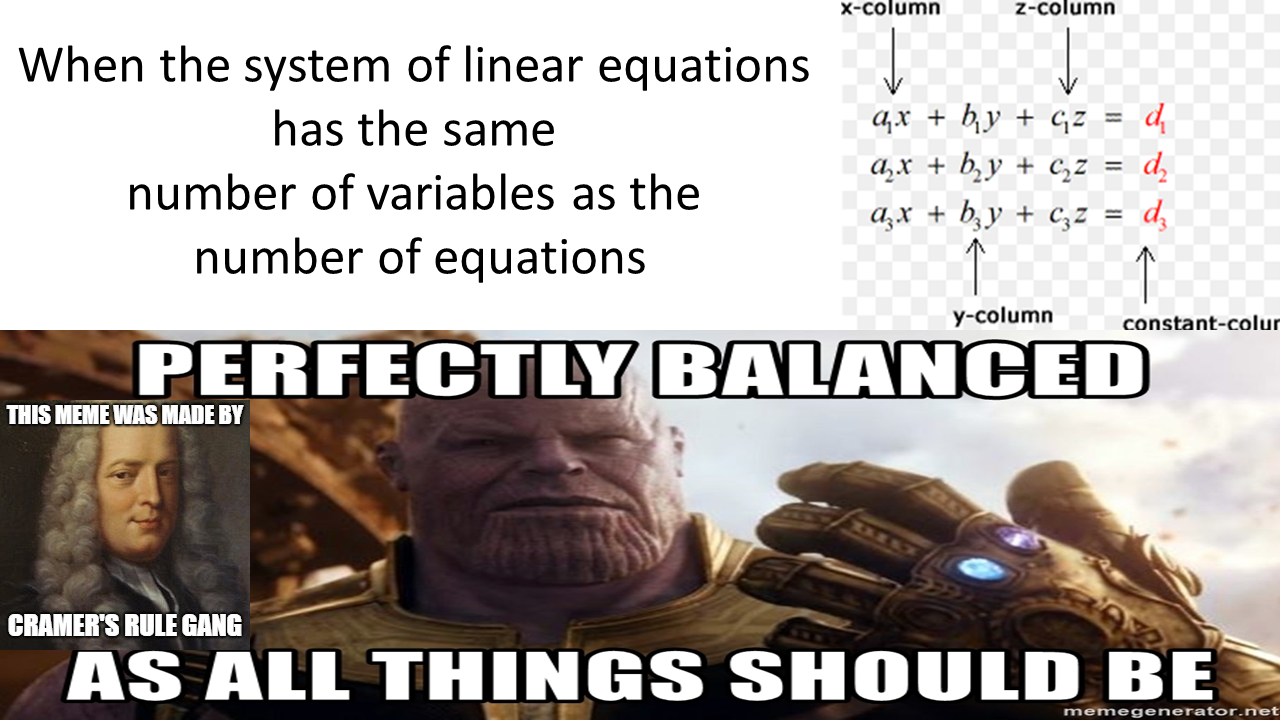
\includegraphics[width=0.5\textwidth]{assets/meme.png}

    \begin{Large}
        Good Luck!
    \end{Large}
\end{center}

\newsection
\section{Exercise tricks}

\begin{multicols}{2}
    $\sin, \cos, \tan$ values ($+\pi \Leftrightarrow x \cdot (-1)$) (to the right)

    \fhlc{red}{IMPORTANT:} For the multiple-choice exercises, try to come up with a short proof for each option

    Non-Trivial null-space $\Rightarrow$ $\text{rank}(A) < n$ if $A \in \R^{n \times n}$

    $A \in \R^{2 \times 2}$ for which $A^{\top} = -A \Leftrightarrow \begin{bmatrix}
            0  & a \\
            -a & 0
        \end{bmatrix}$


    \begin{tabular}[h!]{|c|c|c|c|c|}
        \hline
        \rowcolor{Aquamarine} ° & rad              & $\sin(\xi)$          & $\cos(\xi)$           & $\tan(\xi)$           \\
        \hline
        0°                      & $0$              & $0$                  & $1$                   & $1$                   \\
        \hline
        30°                     & $\frac{\pi}{6}$  & $\frac{1}{2}$        & $\frac{\sqrt{3}}{2}$  & $\frac{\sqrt{3}}{2}$  \\
        \hline
        45°                     & $\frac{\pi}{4}$  & $\frac{\sqrt{2}}{2}$ & $\frac{\sqrt{2}}{2}$  & $1$                   \\
        \hline
        60°                     & $\frac{\pi}{3}$  & $\frac{\sqrt{3}}{3}$ & $\frac{1}{2}$         & $\sqrt{3}$            \\
        \hline
        90°                     & $\frac{\pi}{2}$  & $1$                  & $0$                   & $\varnothing$         \\
        \hline
        120°                    & $\frac{2\pi}{3}$ & $\frac{\sqrt{3}}{2}$ & $-\frac{1}{2}$        & $-\sqrt{3}$           \\
        \hline
        135°                    & $\frac{3\pi}{4}$ & $\frac{\sqrt{2}}{2}$ & $-\frac{\sqrt{2}}{2}$ & $-1$                  \\
        \hline
        150°                    & $\frac{5\pi}{6}$ & $\frac{1}{2}$        & $-\frac{\sqrt{3}}{2}$ & $-\frac{\sqrt{3}}{2}$ \\
        \hline
        180°                    & $\pi$            & $0$                  & $-1$                  & $0$                   \\
        \hline
    \end{tabular}
\end{multicols}


\vspace{-1.5pc}
\subsection{Vector product}
$a \times b = \begin{pmatrix}a_x\\a_y\\a_z\end{pmatrix} \times \begin{pmatrix}b_x\\b_y\\b_z\end{pmatrix} =
    \begin{pmatrix}
        a_y b_z - a_z b_y \\
        a_z b_x - a_x b_z \\
        a_x b_y - a_y b_x
    \end{pmatrix} = c$
gives us a vector $c$ for which $c \perp a$ and $c \perp b$


\vspace{-0.5pc}
\subsection{Basics}
\fhlc{Aquamarine}{Squares of numbers:} $14: 196, 15: 225, 16: 256, 17: 289, 18: 324, 19: 361, 21: 441, 22: 484, 23: 529, 24: 576$
\fhlc{orange}{Long multiplication:} $a \cdot b$, for $n = \text{len}(a), m = \text{len}(b)$ we have $\displaystyle\sum_{i = 0}^{n - 1} \left(\sum_{j = 0}^{m - 1} a[i] \cdot b[j] * 10^{m - 1  - j}\right) \cdot 10^{n - 1 - i}$


\vspace{-0.5pc}
\subsection{Proof patterns}
\newcommand{\pattern}[1]{\shade{Cyan}{#1}}
\begin{enumerate}[label=\textbf{(\Roman*)}]
    \item \pattern{Composition of Implication:} If $S \Rightarrow T$ and $T \Rightarrow U$ are both true, then $S \Rightarrow U$ is true.
    \item \pattern{Direct proof of Implication:} Prove $S \Rightarrow T$ assuming $S$ and then proving $S$ under that assumption.
    \item \pattern{Indirect proof of Implication:} Prove $S \Rightarrow T$ by assuming $\neg T$ and proving $\neg S$ under that assumption.
    \item \pattern{Case distinction:} Prove $S$ by finding a list of $R_1, \ldots, R_n$ (cases) proving at least one $R_i$, then showing that $R_i \Rightarrow S$ for all $R_i$.
    \item \pattern{Proof by contradiction}: Prove $S$ by assuming it to be false, deriving statements from it until reaching a contradiction.
    \item \pattern{Existence proof:} Prove $S$ is true for at least one value
    \item \pattern{Proof by Induction}: Prove $P(0)$ (base case), then prove for any $k$ that $P(k) \rightarrow P(k + 1)$ is true (Induction step). Using an induction hypothesis can be helpful
\end{enumerate}


\vspace{-0.5pc}
\subsection{Proving bijection}
We need to prove surjectivity and injectivity separately.

\fhlc{Aquamarine}{Surjectivity}
Given a function $f: X \rightarrow Y$, it is surjective, iff $\forall y \in Y, \exists x  \in X : f(x) = y$ (continuous function)


\fhlc{Aquamarine}{Injectivity}
$x_1 \neq x_2 \Rightarrow f(x_1) \neq f(x_2)$


\vspace{-0.5pc}
\subsection{Subspace of matrix vector space}
\inlineex \hspace{0mm} $U = \{A \in \R^{2 \times 2} : \text{Tr}(A) = 0\}$. Prove $\dim(U) = 3$. $U \subseteq \R^{2 \times 2}$:

Claim that the standard basis of $\R^{2 \times 2}$ form a basis of $U$, thus implying $\dim(U) = 3$. These are $B_1 = \begin{bmatrix}0 & 1\\0 & 0\end{bmatrix}, B_2 = \begin{bmatrix}0 & 0\\1 & 0\end{bmatrix}$ and $B_3 = \begin{bmatrix}1 & 0\\0 & -1\end{bmatrix}$. Prove that they are a basis by proving that they span $U$.


\newsection
\vspace{-0.5pc}
\subsection{Proof of symmetry}
\inlineex \hspace{0mm} $A \in \R^{n \times n}$ satisfying $AA^{\top} = I$ and $A^2 = I$. Prove that $A$ is symmetric.

$A = AI = A(AA^{\top}) = (AA)A^{\top}= (A^2)A^{\top} = IA^{\top} = A^{\top} \Rightarrow A$ is symmetric


\vspace{-0.5pc}
\newsectionNoPB
\subsection{SVD}
\inlineex \hspace{0mm} $A \in \R^{n \times n}$, $A$ invertible. $\sigma_1$ largest SV of $A$, $\sigma_1'$ largest SV of $A^{-1}$. Prove that $\sigma_1\sigma_1' \geq 1$

Use SVD of $A^{-1}$. From this we know that SV of $A^{-1}$ are given by $\frac{1}{\sigma_1} \leq \ldots \leq \frac{1}{\sigma_n}$ (bc. $\Sigma$ is diagonal). Thus, $\sigma_1' = \frac{1}{\sigma_n}$ (largest SV) $\Rightarrow \sigma_1 \cdot \sigma_1' = \frac{\sigma_1}{\sigma_n} \geq 1$ since $\sigma_1 \geq \sigma_n > 0$


\vspace{-0.5pc}
\newsectionNoPB
\subsection{Least squares}
Least squares is much more versatile than it might seem.
It can even be used for optimization problems in multiple variables or for finding coefficients of quadratic, etc equations. Let's take $ax^2 + b$ as an example. We want to find $a$ and $b$. The $A$ matrix is then simply $1$s on the first column and $x_1^2$, \dots on the second column. Insert the values for $x_1, \ldots$ and compute least squares

\newsectionNoPB
\subsection{Finding values for which a matrix is an inverse for another}
We can interpret a matrix $A^{-1} = \begin{bmatrix}
        \vline & \vline & \vline \\
        x_1    & x_2    & x_3    \\
        \vline & \vline & \vline
    \end{bmatrix}$, then solve SLEs, using $AA^{-1} = I$, whereas $I = \begin{bmatrix}
        \vline & \vline & \vline \\
        e_1    & e_2    & e_3    \\
        \vline & \vline & \vline
    \end{bmatrix}$, where $e_1$ is a standard basis vector. Thus, we get $Ax_1 = e_1$, $Ax_2 = e_2$, \dots

Solving all these SLE gives us solutions for all the variables in the original matrix $A$.


\vspace{-0.5pc}
\subsection{Proving commutativity of matrix operation}
For some matrices, the matrix product is commutative. To prove that, prove that both matrices have linearly independent columns, using the statements from the task and the proof of the first matrix' linear independence. Then finally, show commutativity, e.g. if $AB = I$ and $BA = I$, by showing that $A(BA - I) = 0$


\vspace{-0.5pc}
\subsection{Dimensions of subspaces}
Simply argue with the size of the basis. Thus: Find basis, then argue that the basis specified is actually a basis (by showing that all its elements are linearly independent), then count the number of elements, which is the dimension. \shade{red}{$U_1 \backslash U_2$} can never be a subspace, because $0$ is missing!


\vspace{-0.5pc}
\subsection{Vector combination independence}
\textit{(Other vectors that also form basis)}
Given a basis of a vector space, we have $n$ new vectors, formed form a basis.
To decide if the new set forms a basis, try to construct original vectors from the new ones, or to disprove, show that $0$ vector is a linear combination of the vectors with non-zero coefficients.

\vspace{-0.5pc}
\subsection{CR-Decomposition}
Perform row sign-inversion only at the very end, as it can lead to nastiness along the way. $R$ is in RREF, $C$ the columns with pivot in $R$


\vspace{-0.5pc}
\subsection{Eigenvalues}
For triangle and diagonal matrices, the eigenvalues are on the diagonals. Matrices of all $0$'s are positive semi-definite.

For exercises with a complete set of distinct eigenvalues, we can use the $A = V\Lambda V^{-1}$ decomposition, which for $A^n$ simplifies to $V\cdot \Lambda^n V^{-1}$ and then compute $\Lambda^n$, which is simple because $\Lambda$ is a diagonal matrix (so all entries on diagonal $^n$)
\textbf{Alternate approach}: $\det(A) = \prod_{i = 1}^{n} \lambda_i$ and $\det(A^n) = \det(A)^n$, then check all determinants


\vspace{-0.5pc}
\subsection{SVD}
The pseudo-inverse using the SVD uses the concepts of the SVD with CR-Decomposition. $A = U_r \Sigma_r V_r^{\top}$, where $U_r = C$ and $\Sigma_r V_r^{\top} = R$


\vspace{-0.5pc}
\subsection{Quadratic solution formula}
$\displaystyle \frac{\colorbox{yellow}{-}b \pm \sqrt{b^2 - 4ac}}{2a}$, for $f(x) = ax^2 + bx + c$, result $\R$ iff $b^2 - 4ac \geq 0$. Not that it is strictly needed, but there was still some space. There's an excellent song to remember it: \url{https://www.youtube.com/watch?v=E2eVZFy9yzk}



\vspace{-0.5pc}
\subsection{Multiplying out with transposes}
For vectors, we have $(v - u)^{\top}(v - u) = v^{\top} v - 2v^{\top}u + u^{\top}u$

\newsectionNoPB
\vspace{-0.5pc}
\subsection{Number of Solutions of SLE}
System $Ax = b$ has two characteristic numbers, $m$ (number of equations), $n$ (number of variables). For solution space, we have a third one, $r = \text{rank}(A)$. $A$ in REF doesn't guarantee solution. $A$ in RREF does (in $\R$)!

\bg{red}{Number of solutions}:
\begin{tabular}[h!]{|c|c|c|}
    \hline
    \rowcolor{red}$R_0$ & $r = n$   & $r < n$        \\
    \hline
    $r = m$             & $1$       & $\infty$       \\
    \hline
    $r < m$             & $0$ / $1$ & $0$ / $\infty$ \\
    \hline
\end{tabular}



\newsectionNoPB
\vspace{-0.5pc}
\subsection{Farka's Lemma}
This task is from Assignment 10.
Let $P_1 \subseteq \R^2$, $P^2 \subseteq \R^2$ in the plane.
Assume $P_1 \cap P_2 = \emptyset$.
We want to prove that there exists a vector $v \in \R^2$ and a scalar $w$ such that $P_1 \subseteq \{x \in \R^2 : x \cdot v \leq w\}$ and $P_2 \subseteq \{x \in \R^2 : x \cdot v > w\}$. Intuition: We can draw a line to separate the two polyhedra.

The approach to solve this now, is to assume $P_1 = \{x \in \R^2 : A_1 x \leq b_1\}$ and $P_2 = \{x \in \R^2 : A_2 x \leq b_2\}$ for some $A_1, A_2 \in \Q^{m \times 2}$ and $b_1, b_2 \in \Q^m$ and $m \in \N$.
We observe that the system $\begin{bmatrix}A_1 \\ A_2\end{bmatrix} x \leq \begin{bmatrix}b_1\\b_2\end{bmatrix}$ has no solution since $P_1 \cap P_2 = \emptyset$.
Farka's lemma implies the existence of a vector $y \in \R^{2m}$ with $y \geq 0$, $y^{\top} \begin{bmatrix}A_1\\A_2\end{bmatrix} = 0$ and $y^{\top} \begin{bmatrix}b_1 \\b_2\end{bmatrix} < 0$.


\vspace{2cm}
\begin{center}
    \begin{Large}
        \shade{red}{CHECK FOR SMALL ERRORS!}
    \end{Large}

    These errors could be something like a missing minus. Verify all solutions using computations. 

    \textbf{Example 1:} For Eigenvalues check that $\det(A - \lambda I) = 0$ for all eigenvalues. 

    \textbf{Example 2:} For Eigenvectors check that $Av = \lambda v$ for all eigenvalue-eigenvector pairs. 
\end{center}



\end{document}
